% \documentclass[11pt,a4paper]{article}

% \usepackage[frenchb]{babel}     % specification francaise
% \usepackage[latin1]{inputenc}   % entree clavier latin1
% %\usepackage[T1]{fontenc}        % sortie

% \pagestyle{empty} % pour enlever les numeros de page

% %\usepackage{graphics}
% \usepackage{graphicx}


% % Marges
% % ======
% %\usepackage[francais]{layout}

% \usepackage{geometry}
% \geometry{ hmargin=2.5cm, vmargin=1.5cm }

% % Paysage
% % =======
% \usepackage{lscape}
% %\begin{landscape}
% %notre texte
% %\end{landscape}

% % Multicolonne
% % ============
% \usepackage{multicol}
% %\begin{multicols}{nombre de colonnes}
% %notre texte
% %\columnbreak
% %notre deuxi�me texte
% %\end{multicols}
% %\setlength{\columnsep}{16pt}
% %\setlength{\columnseprule}{0.3pt} 
% \setlength{\columnsep}{16pt}
% \setlength{\columnseprule}{0.3pt}

% \title{Rayons X}
% \author{S. \textsc{CELLES}}
% \date{\null}



% \begin{document}

% %\layout %\usepackage[francais]{layout}


% %\maketitle

% %\begin{landscape}


% %\begin{multicols}{2}

% %Essai

%   \begin{figure}
%     \centering
%     \caption{Le tube de Coolidge}
%     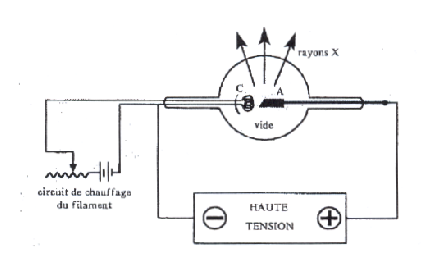
\includegraphics{tube_coolidge.png.eps}
%   \end{figure}

%   \begin{figure}
%     \centering
%     \caption{\'Emission de rayons X par les atomes de l'anticathode}
%     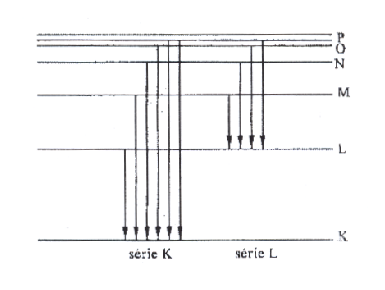
\includegraphics{emission_rayons_x.png.eps}
%   \end{figure}

%   \begin{figure}
%     \centering
%     \caption{Absorption des rayons X par la mati�re}
%     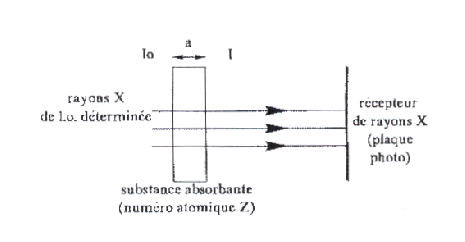
\includegraphics{absorption_rayons_x.png.eps}
%   \end{figure}

%   \begin{figure}
%     \centering
%     \caption{Influence de l'�paisseur travers�e sur l'absorption des rayons X}
%     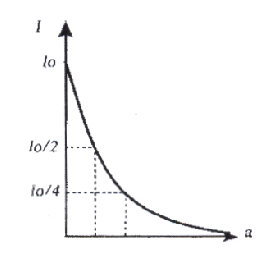
\includegraphics{influence_epaisseur.png.eps}
%   \end{figure}

% %\end{multicols}

% %\end{landscape}


% \end{document}




%%%%%%%


\documentclass[11pt, a4paper]{article}

\usepackage[frenchb]{babel}     % specification francaise
%\usepackage[T1]{fontenc}
\usepackage[latin1]{inputenc}   % entree clavier latin1
\usepackage{capt-of}
\usepackage{lscape}
\pagestyle{empty} % pour enlever les numeros de page

\begin{document}
\begin{landscape}

  \begin{minipage}[c]{0.4\linewidth}
    \centering
    \captionof{figure}{Le tube de Coolidge}
    %\rule{5cm}{5cm}
    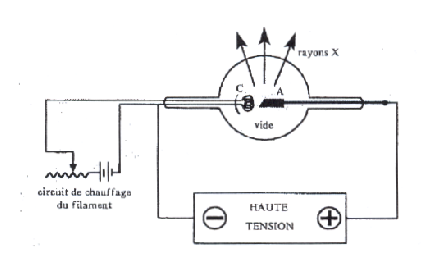
\includegraphics{tube_coolidge.png.eps}

    \vspace{2cm}

    \captionof{figure}{\'Emission de rayons X par les atomes de
      l'anticathode}
    %\rule{5cm}{5cm}
    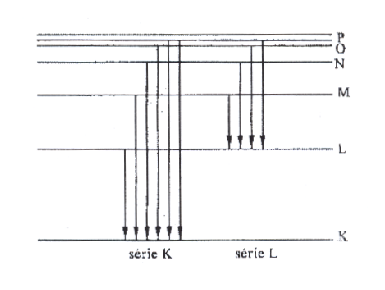
\includegraphics{emission_rayons_x.png.eps}

  \end{minipage}
  \hfill
  \begin{minipage}[c]{0.4\linewidth}
    \centering
    \captionof{figure}{Absorption des rayons X par la mati�re}
    %\rule{5cm}{5cm}
    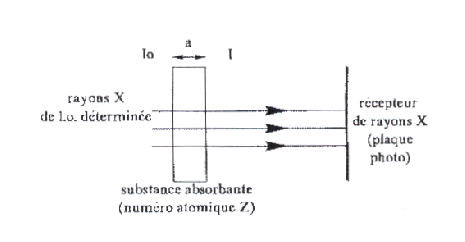
\includegraphics{absorption_rayons_x.png.eps}

    \vspace{2cm}

    \captionof{figure}{Influence de l'�paisseur travers�e sur l'absorption
      des rayons X}
    %\rule{5cm}{5cm}
    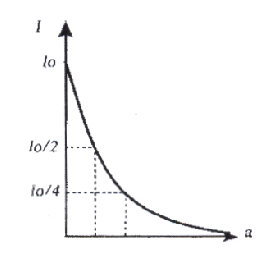
\includegraphics{influence_epaisseur.png.eps}
  \end{minipage}

\end{landscape}
\end{document}